%\documentclass{acm_proc_article-sp} 
\documentclass[11pt]{article} 
\usepackage{amssymb,amsmath} 
\usepackage{graphicx}
\usepackage{float}
\usepackage{hyperref}


\floatstyle{ruled}
\newfloat{code}{thp}{lop}
\floatname{code}{Code}

%\DeclareGraphicsExtensions{.eps}

\begin{document}
	
\title{DBToaster Runtime: System for Streaming Data Processing.}
\author{}
\maketitle

\section{Introduction}

DBToaster application involves three major components. Data Sources components are a source of the incoming data. The end user applications need these data to be processed by running various queries over it. In this particular example we will be using an Exchange Simulation Server application as a data source. Next component is the Algorithms Simulation Engine. This component is the end user program of interest. It is responsible for the decision making and outside influences (i.e. what ever user needs to be done with the help of the queries over the data streams). In out example it is a Trading Runtime Platform. The last component is DBToaster Runtime. The component is responsible for collecting the data from various data sources specified by the users, running appropriate queries over the data and conveying the query results to Algorithms Simulation Engine. 

The the flow of information between the three components is as follows. Once started data generation component generates data, these data comes from a variety of sources stock exchange, sensor network, remote applications etc. The data comes as a continuous stream of information, this information is presented in a well known format. In many of the cases it is possible that the end user does not have much control over the data stream but the ability to listen to the incoming data. These data is sent to DBToaster runtime. The runtime is responsible for collecting data from those data sources and running a dynamic set of user defined queries over these data. The queries are dynamically loaded, compiled and if needed removed during the execution of a runtime. The results of the queries are forwarded to Algorithms Simulation Engine (a.k.a the end user). The Engine's job is to get the data from the runtime. Based on the results of the queries Algorithm Engine performs tasks needed by the users. In our example, based on the information received Algorithm Engine buys and sell stocks on a NASDAQ exchange simulator. 

The particular application we have chosen to demonstrate the capabilities and performance of our system is a NASDAQ trading simulation. In this simulation there is a set of servers; each server arranges stock exchanges between different trading parties. The results of those exchanges as well as information about interest in stock sells and purchases is transmitted to all parties interested in such information. Based on these information different trading algorithms decide to buy and sell stocks. The arrangement of all the components in the Trading system can be seen in figure \ref{TheBigPicture}. 

\begin{figure}
  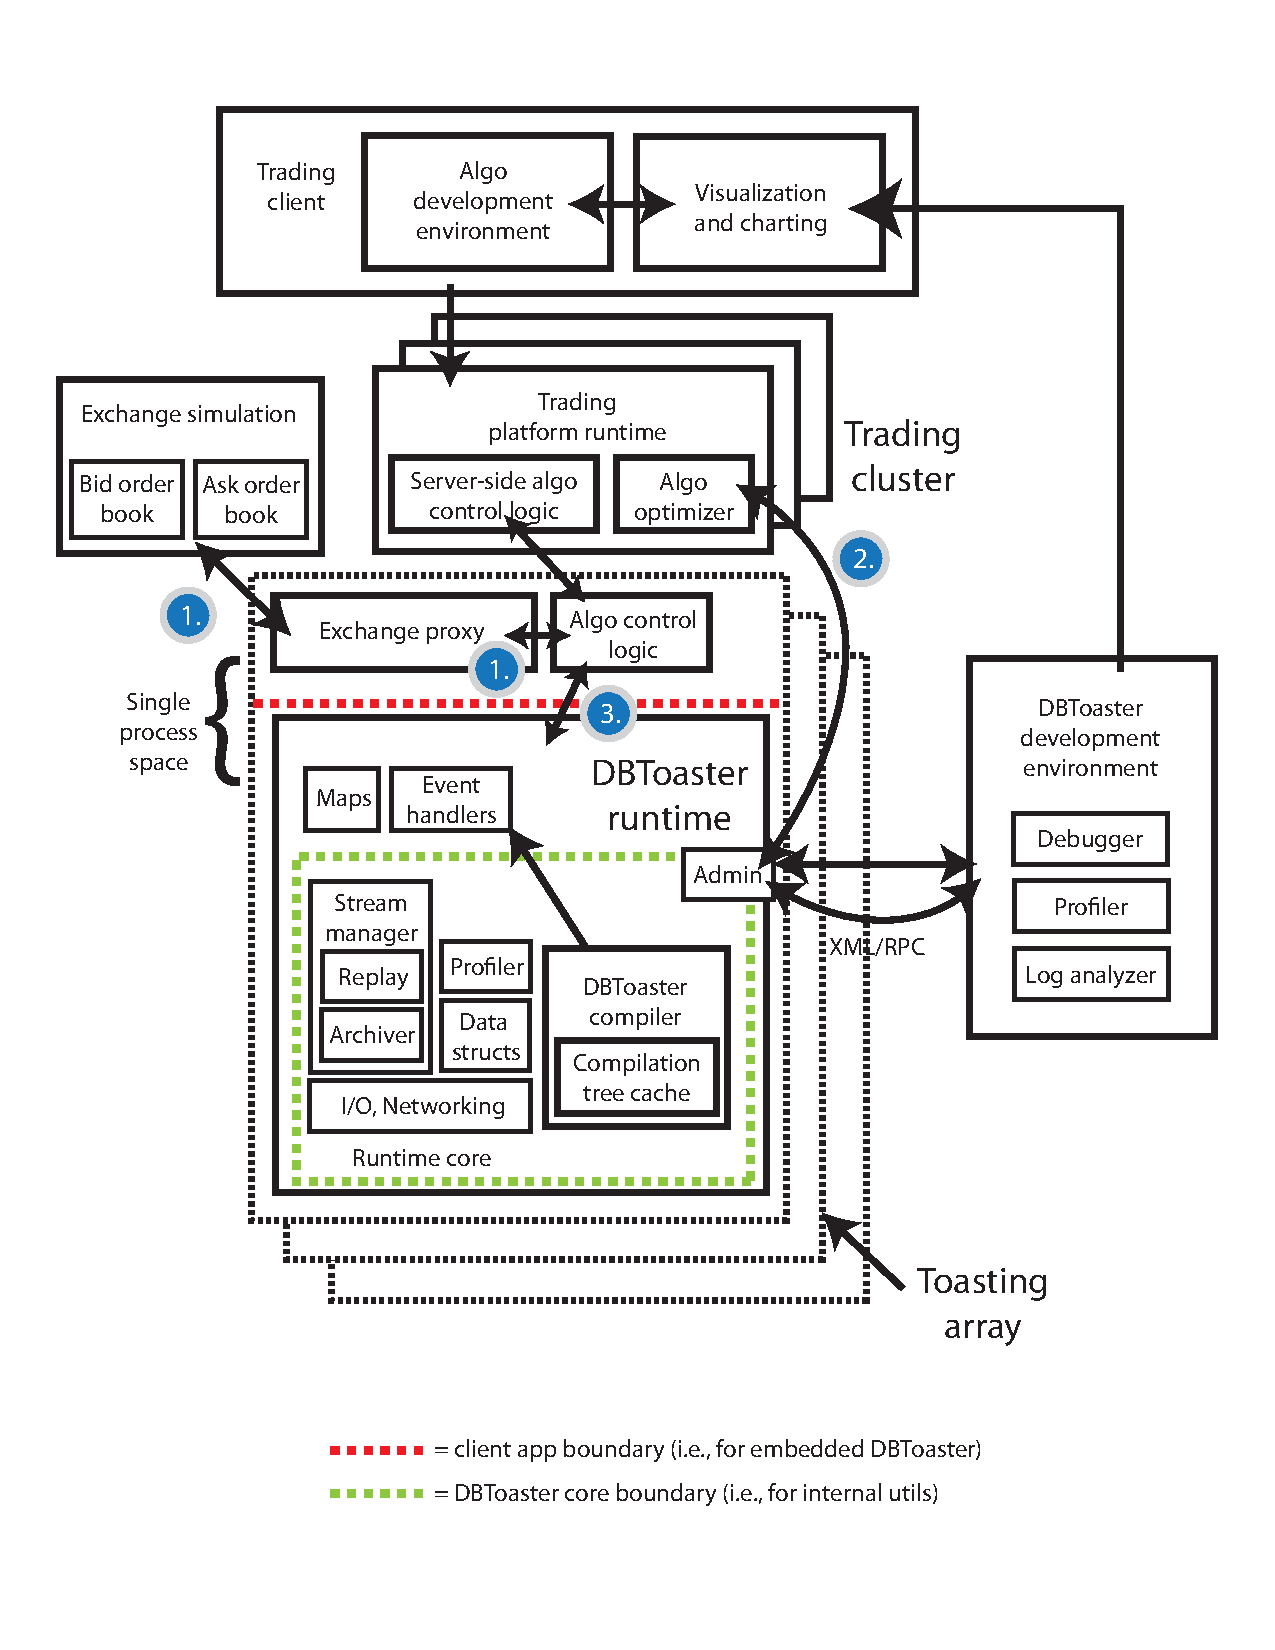
\includegraphics[width=4.50in]{finapp.pdf}
  \caption{Application Overview.}
  \label{TheBigPicture}
\end{figure}

%description of particularities of the system


\section{DBToaster Runtime}

DBToaster Runtime consists of three major components: Compiler, Query Processing and Data Sources Processing. Each of these components interacts with each other as well as has external interactions. The complete representation of DBToaster Runtime can be found if figure \ref{DBToasterPic}. Compiler and Query Processing have a server connection to retrieve relevant data. Data Source Processing creates user specified clients to receive the data from various data sources. Compiler receives requests from the client to instantiate a Data Source Reader to receive data for some queries. The created Reader Client is passed to the Data Source Processor.

\begin{figure}
  \includegraphics[width=4.50in]{DBToasterRuntime.pdf}
  \caption{DBToaster Structure.}
  \label{DBToasterPic}
\end{figure}

\subsection{Compiler}

Compiler consists of several components. Its structure can be seen in figure \ref{CompilerPicture}. Two components responsible or compilation are SQL query pre-compiler and C++ code compiler. 

Compiler is a starting point for all user interactions with the DBToaster Runtime. Once Runtime is up and running the user initiates the contact by specifying that it needs to execute a query on some specific set of data sources. The query, types and parameters of data sources are sent to User Input Handler. It collects the information in a structured format and passes it to the Compiler Admin. Compiler Admin converts a SQL query to C++ code and C++ code to binary format. The query is then passed to the Query Processing Admin to be added to the list of active queries. If the user asks to add a Data Source Reader. The Reader of a specified type is created and passed to the Data Source Admin to be added to the list of active Readers. The Data Adapter is compiled into a binary format and sent to Data Sources Admin to be added to Data Adaptors. 

\begin{figure}
  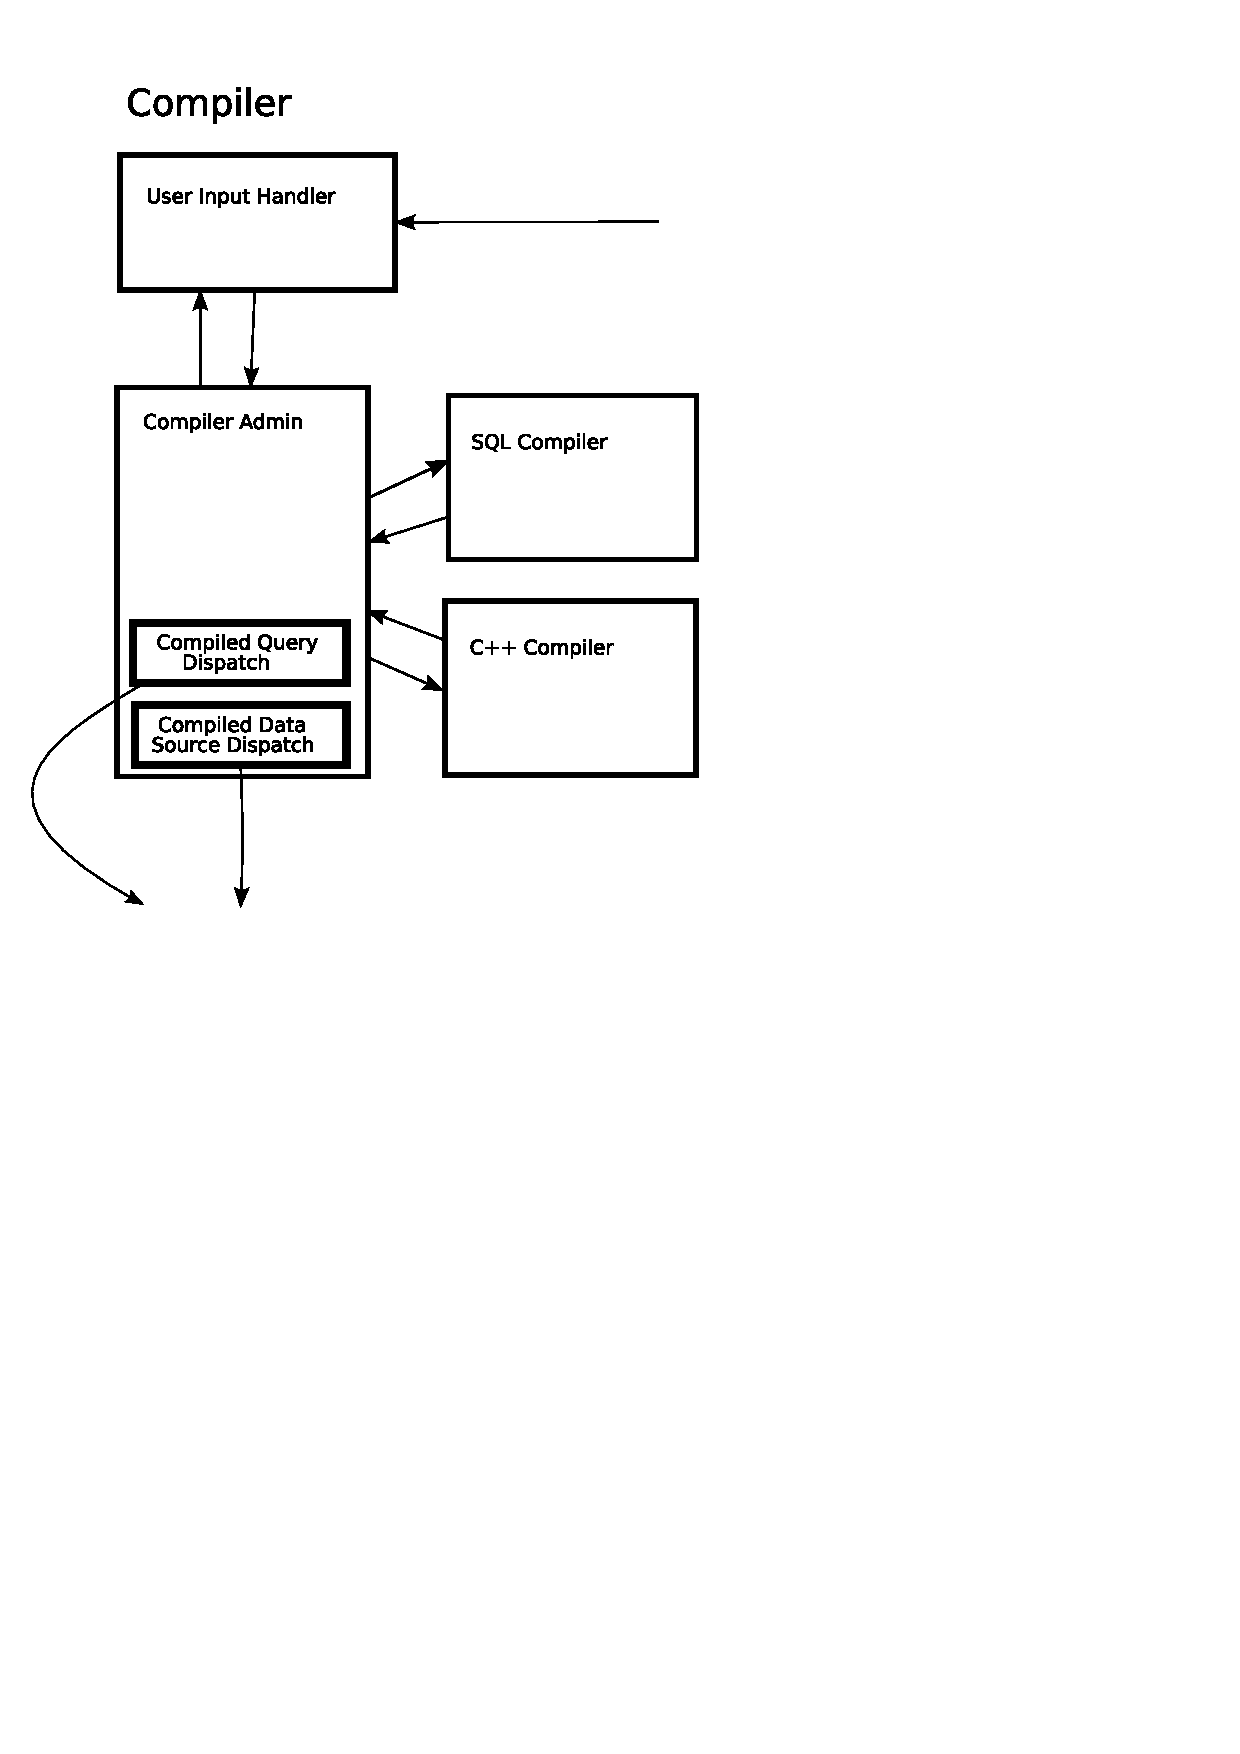
\includegraphics[width=4.50in]{compiler.pdf}
  \caption{Compiler Structure.}
  \label{CompilerPicture}
\end{figure}

\subsubsection{User Input Handler}
The server is implemented as a part of User Input Handler. When a client connects to the Input Handler Server it sends a type of request and attributes of the request to the server:
\\
\\
\begin{tabular}{|l|l|}
  \hline
  Type & Information needed \\ \hline
  Query & Query Source file, list of Data Readers \\ \hline
  Reader & Connection Type, Adapter Source file, list of queries \\ \hline
\end{tabular}
\\
\\*
The two different types of requests are either to add a query or add a data reader.
\\*
Add query request needs the following data from the user:

\begin{itemize}
	\item {\tt AddRequest(type="add query",\\
		 Source="SQL Source File",\\
	     DataReaders="list of Data Readers for Query");}
\end{itemize}

\noindent Add source request is as follows:

\begin{itemize}
	\item {\tt AddRequest(type="add reader", \\
	     AdaptorSource="C++ Adaptor Source file",\\
	     QueryList="list of Queries for information"\\
	     source="IPaddress and port or input file");}
\end{itemize}

This information is then forwarded to the Compiler Admin in a form of a struct:

\begin{itemize}
	\item {\tt Struct InputRequest( type, fileName,\\
	       list<int> informationHandle \\
		   list<string> extraInformation)}
\end{itemize}



\subsubsection{Compiler Admin}

Once user request is received, Compiler Admin takes over. Depending on the type of the request Admin takes different actions. 

On add SQL query request Admin passes the SQL query source file to SQL Compiler. SQL compiler returns a pointer to an containing equivalent to a query C++ file. This file is then passed to the C++ compiler by the Admin. C++ compiler returns a function handle to the compiled binary of the query. The query handle is then passed to the Query Admin to be added to the catalog together with the list of Readers for the query.

On add Reader request Admin passes Data Adaptor file to C++ compiler which in turn returns a function handle to the Data Adaptor. Then Admin creates a Reader and opens a connection for a reader (either a socket or a file). The handle to a Reader together with the handle for a Data Adaptor and a list of queries for this reader is passed to the Data Sources Admin. 

\subsubsection{SQL Compiler}

SQL complier takes a SQL query from a file and creates an optimized C++ coded to be added to the runtime. The file name containing the code is returned to the Admin.

\begin{itemize}
	\item {\tt cCodeFileName CompileSQL(SQL file name);}
\end{itemize}

\subsubsection{C++ Compiler}

C++ compiler takes file containing C++ code. C++ compiler creates a binary code version of the code and returns a function handle of it to Admin. \emph{not sure about the return form. it is possible we need to return several function handles ... not sure yet}

\begin{itemize}
	\item {\tt functionHandle CompileC++(C++ file name);}
\end{itemize}

\subsection{Data Source Processing}

Data Source Processing is done in series of steps. Once Data Sources Admin receives a function handles from Compiler Admin. The Reader handle is inserted into Collection of Data Readers. Each reader gets the data stream from outside. The handle for the Reader is for a function {\tt getNext()}.

The Data Readers Thread Pool is a collection of threads where each thread picks a Data Reader and executes a read at a time from one of them. Once read is done the results of the read are forwarded to a Data Structure Dispatch. The Dispatch uses the appropriate Data Adapter to handle the data into a structured format, then the structured data is forwarded to Query Processor, in particular to the Query Tuple Queue. The more pictorial description can be found in figure \ref{DataSourcePic}.

% processing consists of the list of list of stream points. Each point is given by the user and signifies a way for a DBToaster to connect with the input stream of some process which dispatches data to the DBToaster. Each Stream Point is written by the user and user can fully specify how the data should be received and processed. Stream point is responsible for sending data to the Data Dispatch unite in a pre-specified format. The structure for data source processing can be found in figure 

\begin{figure}
  \includegraphics[width=5.00in]{DataSources.pdf}
  \caption{Data Sources Management.}
  \label{DataSourcePic}
\end{figure}

\subsubsection{Data Sources Admin}

Data Sources Admin receives two function handles one to a data Reader and another one for a Data Adaptor from a Compiler. First Admin locks Data Adaptors and inserts a new Data Adaptor. Then Admin locks Data Readers Queue  and a handle is inserted. Each Data Readers handle implements a method \emph{readNext()} for reading data from some data source (typically a socket or a file).

\begin{itemize}
	\item {\tt rawDataTuple getNext();}
\end{itemize}

\noindent The {\tt rawDataTuple} is a pair {\tt <size, bit-string>}.

The Reader extracts the informations from either a file or a socket. Reader's communication with the outside world is in a standard format. On a request it reads a header from the input stream with the size of the message and then reads the message of the given size. The size and message is then forwarded to further. \emph{TODO: expand this into a section with the full description of Readers input formats}.

\subsubsection{Data Readers Thread Pool}

Data Readers Thread Pool is a collection of identical threads. Each thread is responsible for getting a reader from the queue of Data Readers, executing a \emph{readNext()} message, collecting the message {\tt rawDataTuple} and sending it to Data Structures Dispatch together with the ID of a Reader.

\subsubsection{Data Structures Dispatch}

Data Structures Dispatch receives an ID identifying each Data Reader and a message read by the reader. 

\begin{itemize}
	\item {\tt structuredTuple DataStructuresDispatch(readerID, rawDataTuple);}
\end{itemize}

Based on the ID of a reader Dispatch Calls for on an appropriate Data Adaptor to convert the incoming {\tt rawDataTuple} message into a structure needed by the query. The structured tuple is then sent to an appropriate set of queues in the Data Queue for Processing. The {\tt structuredTuple} is a pair {\tt <size, bit-sequence>} such that the bit sequence can be interpreted by the query. 

\subsection{Query Processing}

Query Processing is done mostly in Query Executor with a set of Query Threads each thread picks a query-datum pair from a pool of available pairs and processes it. As data comes in after been processed it is sent to the appropriate query. As soon as the query receives a datum it becomes available for execution. The structure for query processing can be found in figure \ref{QueryProcessingPic}.

\begin{figure}
  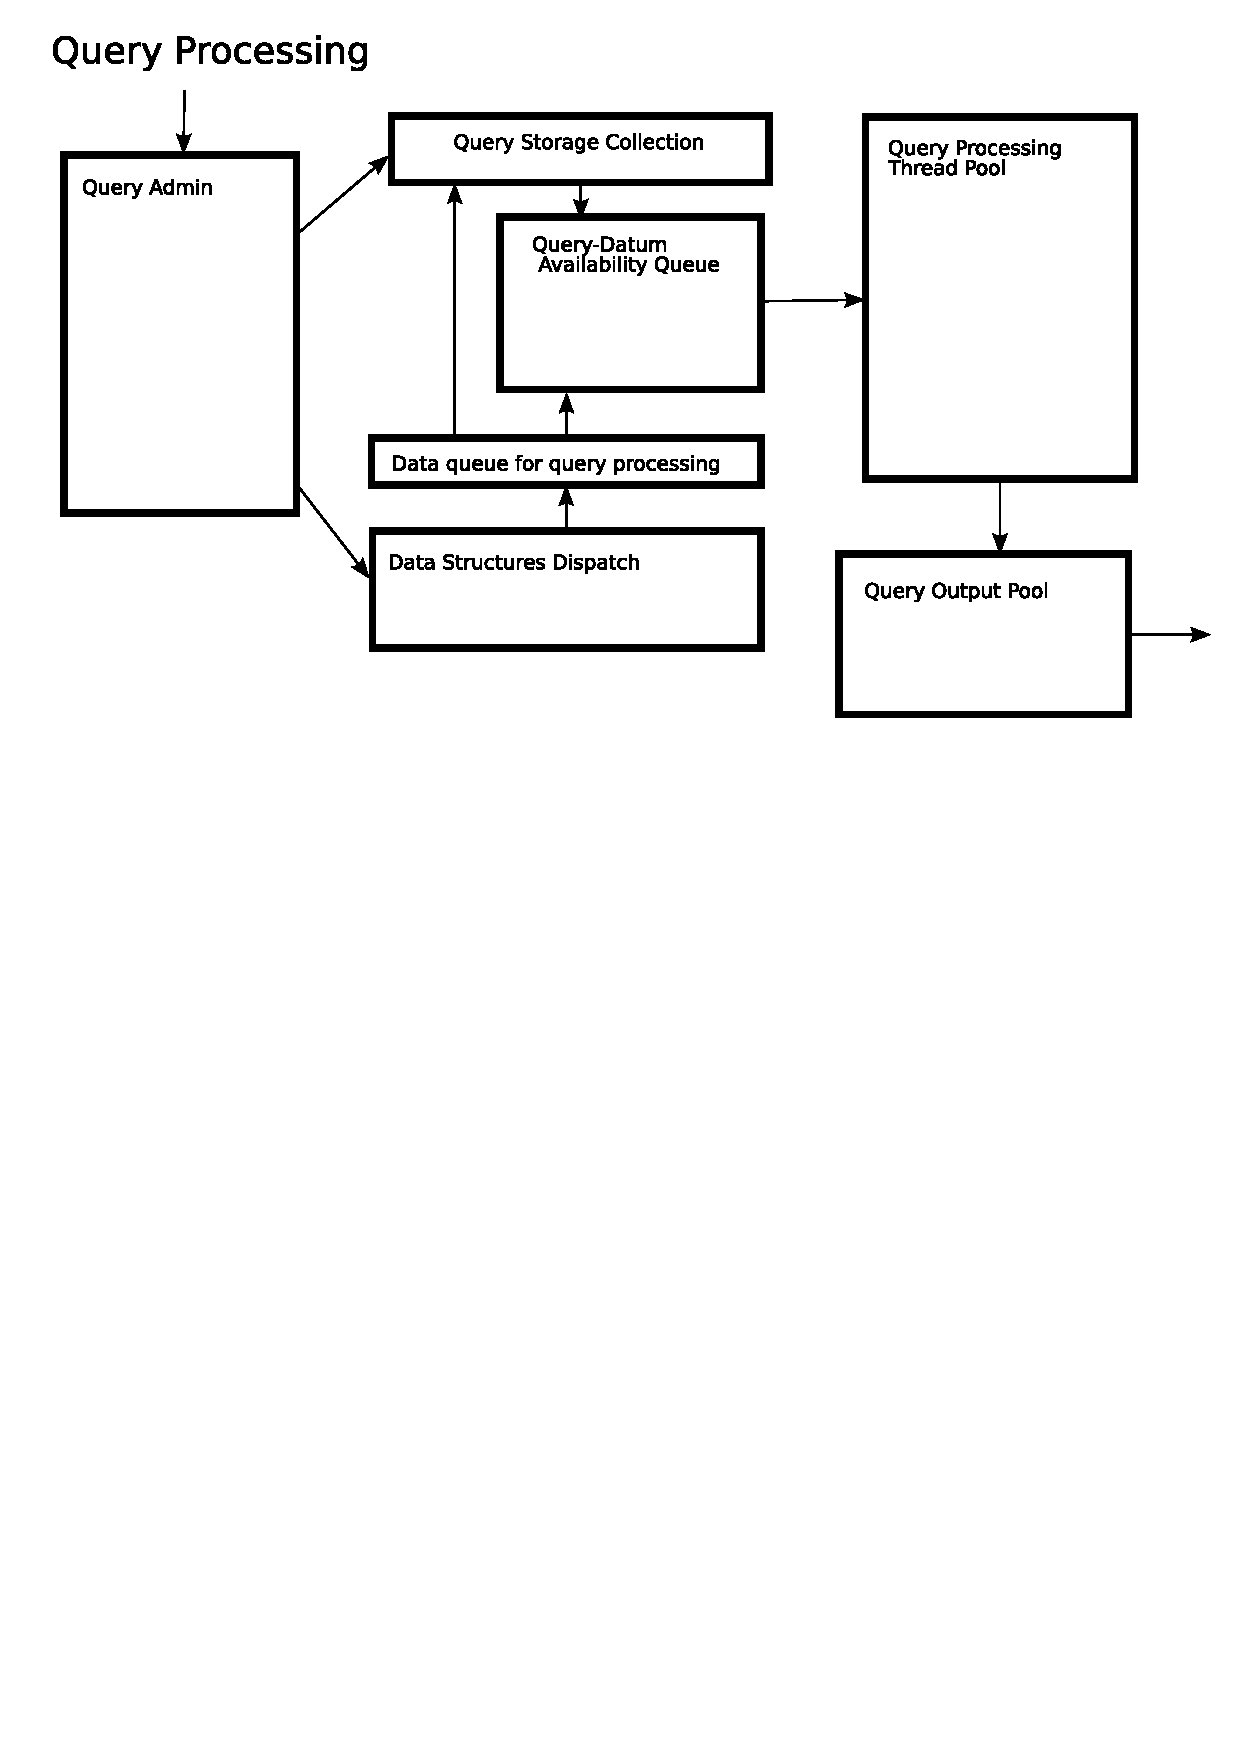
\includegraphics[width=5.00in]{QueryProcessing.pdf}
  \caption{Query Processing Management.}
  \label{QueryProcessingPic}
\end{figure}

\subsubsection{Query Admin}

Query Admin receives a function handle to query. It also receives a list of the readers IDs for that query. Once the handle is received Admin locks Query Catalog and inserts the query there, then Query Results Queue is locked and updated to have an output queues for just inserted query. Finally Admin locks Query Tuple Queue and inserts and additional queue for data associated with the query. 

Query Catalog is a map containing query ID and a handler for that query. 

\subsubsection{Query Tuple Queue}

This is a collection of queues. Each queue in the collection corresponds to the query that can run data items in the queue. When Query Tuple Queue receives a new item, from Data Structures Dispatch, together with the ID of the data Reader the {\tt structuredTuple} in inserted into appropriate queues of the queries which need this data.  If the query queue is empty when the data item is inserted the query handle is extracted from the catalog and inserted in the scheduling queue. Scheduling Queue contains handles of the queue with the data items which are ready for them. If the query is running the item is inserted into queue.

\subsubsection{Query Processing Thread Pool}

Query Processing Thread Pool is a set of identical threads. Each thread is responsible for picking up and query handle from Scheduling Queue. Then thread runs a query on the datum on top of the appropriate query queue in Query Tuple Queue. The results are put into a Query Results Queues; into a set of queues for the users which are interested in the results of this query. 

\subsubsection{Query Results Queue}

Query Results Queue implements a server, where each client upon connection indicates a set of queries they are interested in.

\begin{itemize}
	\item {\tt userDataStructuresDispatch(userID, Query ID list);}
\end{itemize}

\noindent The server creates a map of query IDs and query result queues for each client. When a query produces an output, it is sent to the Results Queues. In the Result Queues the query results are dispatched to the appropriate queues.

\begin{itemize}
	\item {\tt queryDataStructuresDispatch(queryID, structuredTuple);}
\end{itemize}

\noindent When a client needs a new piece of information it sends a request to the server with the ID of a query it is interested in and the number of tuples it needs. Server returns the results of the query indicated by the ID and the tuples it produced. 

\section{Data Generation}

Data can come in a variety of forms. For our particular application we have developed an Exchange Simulation Server. The server is responsible for processing and broadcast of all stock exchanges to the clients that are connected to it. Server can also is capable to augment data flow by adding data from files containing historical traces of real stock exchanges. At the moment the Exchange Server designed to simulate trade exchanges for one stock.   

\subsection{Exchange Server Simulator}
ExchangeServer creates server port and handles all incoming client connections. Each connected client is given it's own thread (ExchangeThread). ExchangeServer also creates a DataThread, which is responsible for reading historic trace data. The server also creates structure for datastorage which is shared by all of the clients.

\begin{code}
  \begin{verbatim}
Server_socket;
SynchronizedBooks DataBook;
Data_socket(inputDataFile.cvs);

while (Server_socket.listen)
{
	get(client);
	run(client, DataBook);
}
  \end{verbatim}
  \caption{ExchangeServer: inputDataFile.cvs}
\end{code}



\subsection{Exchange Thread}
On a client connection Server creates an ExchangesThread to deal with client needs. All ExchangesThreads share data storage structure DataBook as well as a list of all currently active clients. On a start up thread expects to receive a message from a client indicating the type of a client.
\\
\\
\begin{tabular}{|l|l|}
  \hline
  \multicolumn{2}{|c|}{Client type} \\
  \hline
  0 & Interactive\\ \hline
  1 & Passive Listener \\
  \hline
\end{tabular}
\\
\\*
\emph{Interactive} clients send data and are only interested in receiving messages in response to their transactions. \emph{Passive Listener} clients are interested in all of the transactions but tend not to send the messages themselves.

The messages from clients are coming in the pre-specified format. Depending on the client's request several actions occur:
\\
\\
\begin{tabular}{|l|l|}
  \hline
  Request & Action \\ \hline
  'B' & buy request, check ask book for match if no add to bid book \\ \hline
  'S' & see request, check bid book for match if no add to ask book \\ \hline
  'D' & delete request from appropriate book if one exists \\ \hline
  'X' & cancel order remove trade request from appropriate book\\
  \hline
\end{tabular}
\\
\\
Each transaction is announced to all Passive Listeners as well as to Interactive client which intiated the transaction. 

% the first  message showing an interest in exchange ExchangesThread checks if there is an appropriate match in the data structures (i.e. if some one wants to sell some amount of stocks the thread will look if someone wants to buy stocks at the given price), if so the match is executed if not the request is stored in the data structures. The results and the transaction are announced to all the connected clients. 

\subsection{Data Storage}
SynchronizedBooks is a shared data structure. It is shared between all of the clients. Each client can modify it by adding/removing buy/sell requests. The data structure consists of two SortedBooks. Each SortedBook is a structure that has properties of a sorted set and a hashtable. 

When an addition of a sell/buy request is invoked data structure tries to find a matching buy/sell request and if found the update message is sent to the clients additionally to the original sell/buy request. The update message contains information about the fact that one or both of the orders are partially/fully satisfied. The exchange message is of the form:
\\
\\
\begin{tabular}{|l|l|}
  \hline
  Request & Action \\ \hline
  'E' & order number, update amount \\ \hline
  'F' & order was executed in full \\

  \hline
\end{tabular}
\\

\subsection{Data Generation}

ExchangeServer is capable of augmenting the data flow between clients with the additional data from historical data files. To accomplish this goal server has a DataThread. It can be initiated at any point by a server (for example, once there is a client connected to the server). DataThread reads a historical trace file in a .cvs format and transmits each message to the server as if it was a real request.


\section{Algorithms Engine}

Algorithm Engine code developed by the end users. The code makes use of DBToaster Runtime to query the continuous data from input streams specified by the users. The query results are then processed by user defined algorithms to achieve their goals. 

In our example Algorithmic Engine creates and runs a set of monitoring queries for the stock trading depending on the results of the queries and the internal mechanics - algorithms decide to buy or sell stocks on a NASDAQ Trading Exchange Simulator.

\subsection{Data Sources}

Algorithmic Engine interacts with environment in three different ways. First of all the Engine needs to receive  the information from from DBToaster runtime. This interaction is unavoidable since the Engine needs the results of the queries. Another interaction which needs to be added is the way to specify the information stream received by a DBToaster runtime. This information needs to be passed the the Runtime in the form of c++ code for the Runtime to compile. Another optional source of interaction is infulencing the enviroment. In our example is the Engine's capability to add/remove stock requests from the Exchange Server. 

\subsubsection{Data Stream}

There are two interactions with outside systems needed to be implemented by the user. The first interaction is with DBToaster. A system needs to pull information from the DBToaster runtime. \emph{TODO description of the the pulling mechanism}.

Another interaction, which needs to be passed to the DBToaster Runtime, is a way for Runtime to access the data streams relevant to the Engine and over which the queries needed to be post. This information is specified as a C++ code which is sent for the compilation to the Runtime to be added to the system.

\subsubsection{External Influence}

If the Engine implements interactive process, which needs to access outside processes or interact (influence) them then this is interactivity needs also to be added. In our example Algorithmic Engine can buy and sell stock on our Exchange Simulation Server. Thus acting like one of the clients of the server. \emph{TODO describe the system in more details}

\subsection{Algorithm}

This is the part which is the most relevant to the user and will vary from system to system. In out example we encoded the learning and trading strategies for NASDAQ stock exchange. \emph{TODO describe the system in more details}

\subsection{Query creator (or something like that)}

Queries posed to the DBRuntime can come from various sources they can either be predefined by the user system or written and modified dynamically. In order to be active they need to be passed to the Runtime where they are compiled and added to stream observations. \emph{TODO describe the process more}



\end{document}





